%*****************************************
\chapter{Related Work}\label{ch:related_work}
%*****************************************
%\setcounter{figure}{10}
% \NoCaseChange{Homo Sapiens}

Researchers studying Ubicomp environments have typically been facing one common problem: evaluating the system. This is because to set up the targeted environment requires space, money and a lot of time; and even if they have access to the whole infrastructure, sometimes is almost impossible to experiment on real case scenarios because of the technological limitations on gathering the contextual data required by the targeted system. Even if all these challenges are overcome, real and large scale experiments are really expensive, hence only a limited number can be conducted.\\

To address these issues, a number of projects have tried to develop simulation tools and frameworks in various research areas, some of them being generic, others being more targeted towards a certain domain.\\

In this chapter I will present the work in this area I found most relevant and inspiring for my thesis.

% %BEGIN: Service in Smart Homes
\section{Services inside the Smart Home: A Simulation and Visualization tool}\label{sec:services_in_smart_homes}

In this work \cite{lazovik2009services} the aim was to reduce the testing costs of smart homes. The goal was achieved by implementing a simulation and visualization tool which replaces services in a smart home with virtual stubs behaving just like the real hardware installed in a house. The resulting simulation tool is called ViSi.\\

The simulation scenarios were built using Google SketchUp \cite{sketchup:online}. This was enhanced with a set of tools extending its visual representation of a house with virtual home interactive web services supporting SOAP messages. Further, the visualization component was written as a set of plug-ins for Google SketchUp.\\

\begin{figure}[H]
	\centering
	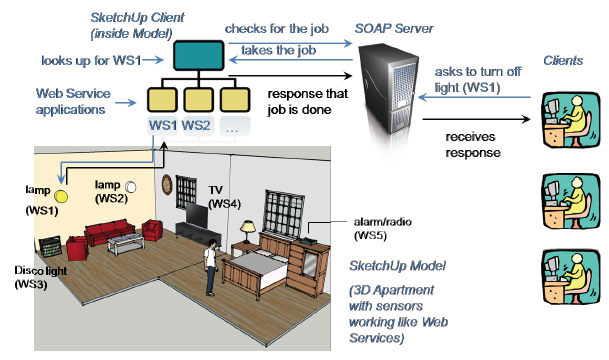
\includegraphics[width=\linewidth]{gfx/Chapter2/services_in_smarthomes}
	\caption{Architecture of the domotics simulation environment ViSi.}
	\label{fig:diasim_architecture}
\end{figure}

The simulation and visualization tool allows to simulate any possible home automation scenario, with the possibility of modelling the user and its interactions with the home.
%END: Service in Smart Homes

%BEGIN: Simulation of Smart Environments
\section{Simulation of Smart Environments}\label{sec:sim_of_smart_envs}

Armac and Retkowitz developed a tool called \emph{eHomeSimulator}, which was build in order to support the simulation of smart environments, or as the authors refer to them in the present work \emph{eHomes} \cite{armac2007simulation}. The motivation behind the work is that smart environments constitute already an important research area, but building a real eHome is associated with high effort and financial costs. Therefore, the eHomeSimulator helps in abstracting out from creating buildings (the actual physical environment) and purchasing devices, allowing the researcher to focus only on software engineering aspects and challenges involved in eHome development (e.g. developing services, deployment, etc).\\

Describing in details the eHome is out of scope, but for clarity, I will a offer a short description. eHome is basically a framework consisting of a hardware platform (the residential gateway) and a software platform (service gateway, runs on top of the hardware platform). The devices and appliances, which make up the eHome, are connected to the hardware platform. They are of two basic types: sensors and actuators. Sensors offer contextual information like temperature, humidity, etc; while actuators can change the environment's state (e.g. a speaker, a heater). The hardware platform is governed by the software platform which acts as a runtime environment for eHome services. These services can be of two types: basic and integrating. Basic service are meant to control devices (e.g. a lamp driver) while the integrating services are composed of various basic service. These services are developed based on the OSGi component model \cite{allianceosgi}, imposing a highly decoupled architecture to the service model and offering high reusability of the developed services.\\

The eHomeSimulator was built on top of the eHome framework to allow intuitive interaction and to visually represent the state of the simulated environment. In the evaluation process of the simulator, eHome environments consisted of three main elements: rooms, devices and persons (agents interacting with the environment). The graphical representation was a 2D view with a view point from top, which is built up from three layers:
\begin{itemize}
	\item The bottom layer contains the graphics to represent the background (floor, walls and furniture) build up from tiles placed one next to each other.
	\item On top of the background, there is the middle layer representing the graphics of the devices. These are only static devices and they can have different colours based on their state.
	\item The top layer represents the agents interacting with the environment. They can move freely in all accessible areas, interacting with the devices.
\end{itemize}

There is an environment editor which assists in setting up a simulated environment. The process starts by designing the room, walls and furniture using Google Sketchup \cite{sketchup:online} which then is uploaded into the editor. On top of this base we can further place the devices and appliances.\\

The eHomeSimulator's architecture is based on the Model View Controller design pattern \cite{erich1995design}. The model of the system holds the data structures representing the current state of the system, the view implements the graphical representation based on the current model and the controller process the user interaction with the simulator, updating the view according to changes in the model.\\

The image depicted in Figure \ref{fig:simulated_env} displays a simulation in progress. On the right side, we can observe the agent interacting with the environment while on the left side there is a control panel displaying contextual data of the monitored entities and allows to interact with nearby devices (e.g. turn on/off a lamp).

\begin{figure}[H]
	\centering
	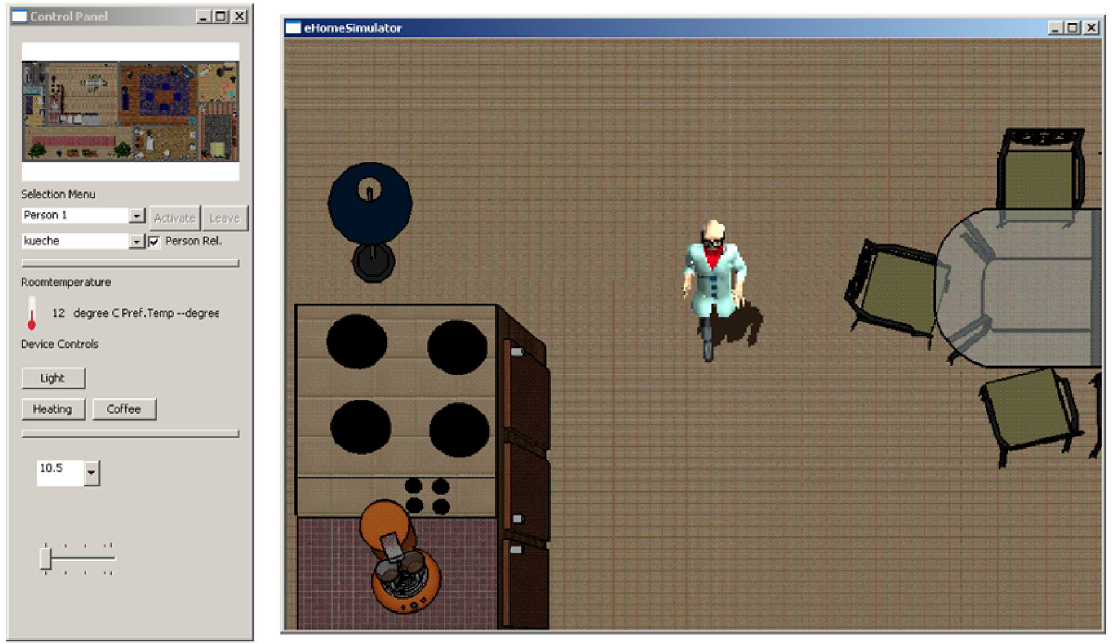
\includegraphics[width=\linewidth]{gfx/Chapter2/simulated_env}
	\caption{The GUI of the simulator}
	\label{fig:simulated_env}
\end{figure}

The framework allows to simulate only sensors and devices. Physical objects are passive and unidentifiable, they are part of the first layer, the bottom layer containing the graphics to represent the background (floor, walls and furniture).\\

As for interacting with the simulated environment, the user can manipulate the agent (the virtual avatar), to walk around in the 2D environment. Given the nature of the visualization, the agent can be facing four directions: forward, backward, left or right. Sensor and devices are activated on a per room basis, not on actual proximity to each individual entity. Devices in the current room can be operated through the \emph{Control Panel} (e.g. turn lamp on/off).\\
%END: Simulation of Smart Environments

%BEGIN: SIMACT
\section{SIMACT}\label{sec:simact}
\emph{SIMACT: a 3D Open Source Smart Home Simulator for Activity Recognition with Open Database and Visual Editor.}\\

SIMACT is a smart home infrastructure simulator, developed in Java, designed to help researchers working in the field of activity recognition \cite{bouchard2012simact}. This work is specifically focused on the interaction between an agent and the surrounding environment in the smart house. It is built to reproduce everyday life scenarios, on a step-by-step basis.\\

The simulator was built entirely on Java based technologies. The GUI was based on the swing library, while the 3D renderer was based on the Java Monkey Engine (JMonkey) version 2.0 \cite{jme:online}. For the 3D design, they have used a modelling tool for house design and interior accessories from Google called SketchUp\footnote{\url{http://www.sketchup.com}}.\\

To further detail, we will briefly discuss on the system's architecture, as illustrated in Figure \ref{fig:simact_architecture}.

\begin{figure}[H]
	\centering
	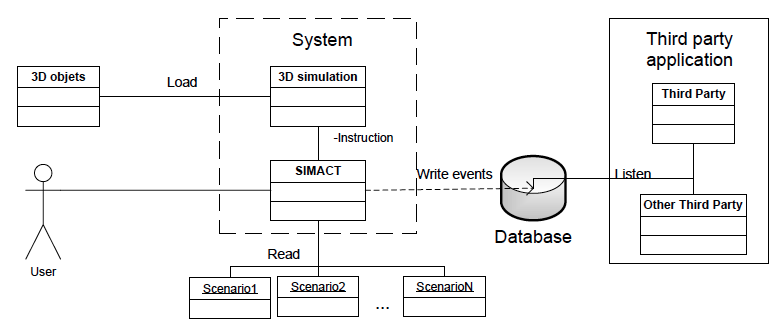
\includegraphics[width=\linewidth]{gfx/Chapter2/simact_architecture}
	\caption{SIMACT: System Architecture}
	\label{fig:simact_architecture}
\end{figure}

To create a custom simulation, a researcher starts out by defining the environment and the object models contained within. The simulator loads these definitions to create the virtual model of the environment and to initialize the 3D simulator. To define the interaction with the habitat, the researcher provides the simulator with an XML file defining the interaction scenario. The scenario is defined as a sequence of steps, which is read, interpreted and execute by the simulator (it plays the role of an interpreter). As the steps are executed and the environment gets modified by these actions, the generated events are written into a database. Further, third party applications can communicate with the database to retrieve data in real-time, which can be used in the logic of the application.\\

A snapshot of the simulation tool in action is depicted in Figure \ref{fig:simact_simulation_tool}.

\begin{figure}[H]
	\centering
	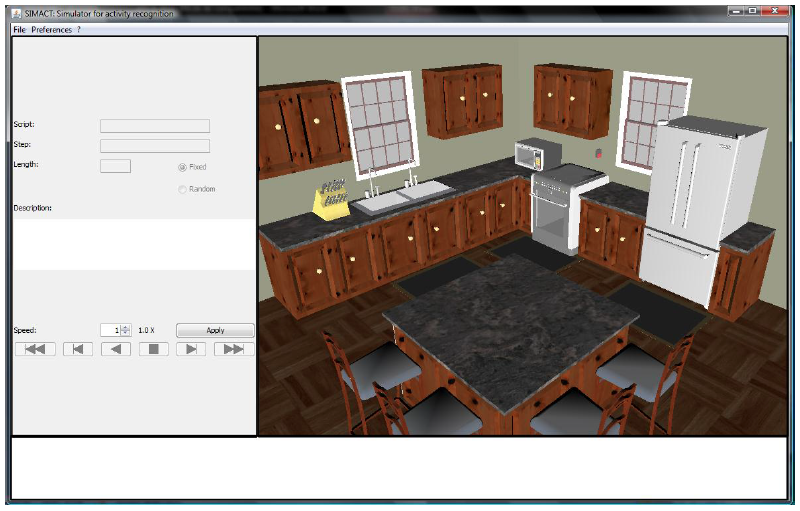
\includegraphics[width=\linewidth]{gfx/Chapter2/simact_simulation_tool}
	\caption{SIMACT: Simulation Tool in Action}
	\label{fig:simact_simulation_tool}
\end{figure}

The novel approach in this simulator is that entire scenarios and interactions can be designed only by using scripts and visual editors, without having to write one line of code. For the 3D design, the researchers have used a modelling tool for house design and interior accessories from Google called SketchUp. This comes with the advantage of a community maintaining a library of free 3D models, where one can find many accessory that would fit in a home.\\

The framework enables simulation of both devices and physical objects. The entire simulation is controlled by the framework as it interprets the simulation scenario, described in an XML file. This is a step-by-step description of how various parameters of the system (e.g. the temperature in a room) and of objects (e.g. door opened/closed, lamp on/off) evolve. During the simulation, context data can be retrieved by third party service from the data base exposed by the framework.\\

The 3D visualization is a simple animation of the simulation allowing the researcher to look around within the ongoing simulation to better observe the evolution of the system. ''In the 3D zone, one can freely move the camera around the environment to take different points of view and then decide where is the most appropriate position to see what is going on. It is simply done by clicking on the frame and using a keyboard: the arrow keys to rotate and pg up/pg down to zoom'' \cite{bouchard2012simact}.\\

The framework's source code is publicly available as open-source.
%END: SIMACT

%BEGIN: DiaSim 
\section{DiaSim}\label{sec:diasim}
\emph{DiaSim: A Parameterized Simulator for Pervasive Computing Applications.}\\

DiaSim is a Java based simulator for pervasive computing applications based on sensors and actuators \cite{bruneau2013diasim}. In this project, the simulation process starts out by defining a high-level description of the target pervasive computing environment, in a domain specific language: DiaSpec. Part of this definition are \emph{classes of entities} and \emph{data types} which can be exchanged by the entities. Based on this definition, DiaGen produces a customized \emph{programming framework} and an \emph{emulation layer}.\\

\begin{figure}[H]
	\centering
	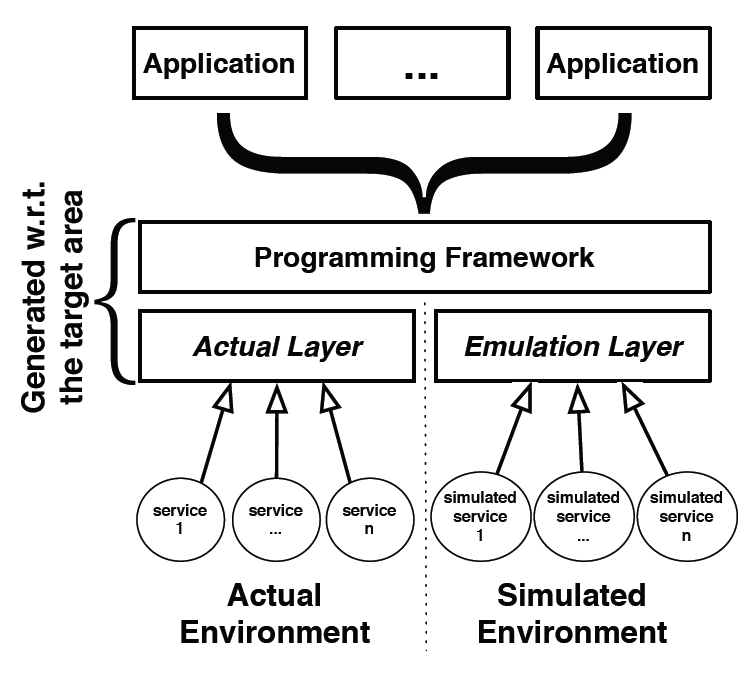
\includegraphics[width=\linewidth]{gfx/Chapter2/diasim_layered_architecture}
	\caption{DiaSim layered architecture}
	\label{fig:diasim_architecture}
\end{figure}

As depicted in Figure \ref{fig:diasim_architecture}, the simulator has a modular, layered architecture. Applications written using the generated programming framework, can be run both in a simulated and a real-world environment. In the real environment, the data comes from real sensors, while in the simulated environment the data comes from simulated sensors in the emulation environment. Besides the components mentioned so far, DiaSim also includes a simulation renderer, enabling the researcher to visually monitor and debug the pervasive computing system.\\

At the heart of this simulator, is the simulation model. The core entity is called a \emph{stimuli}. This represents changes of the environment observable by the sensors in the system. Entities that generate stimuli are called \emph{stimulus producers}, producing only one type of \emph{stimulus}. The generated stimuli may trigger sensors (e.g. a motion detector) which publish events, that may in turn stimulate actuators or services. Making an analogy in object-oriented programming, stimulus would be a class, stimuli would be an instance of that class and the stimulus producer would be a factory \cite{gamma1994design}, producing instances of the stimulus class based on a certain set of rules. These rules define the evolution of the stimuli in terms of space, time and intensity (e.g. an agent moving from one location to another). Each stimulus has a type associated with it, matching the type one at least one sensor in the system.\\

\begin{figure}[H]
	\centering
	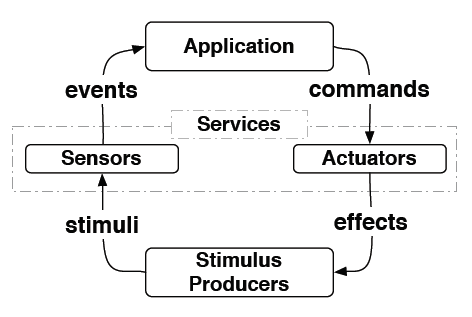
\includegraphics[width=\linewidth]{gfx/Chapter2/diasim_simulation_model}
	\caption{DiaSim simulation model}
	\label{fig:diasim_simulation_model}
\end{figure}

As illustrated in Figure \ref{fig:diasim_simulation_model}, besides stimulus producers, the simulated environment also contains simulated services; they process stimuli, perform actions and interact with other services. The two key services in this simulator are \emph{sensors} and \emph{actuators}. The interaction between services and the environment are based on one of the existing three interaction modes:
\begin{itemize}
	\item Command (one-to-one, synchronous interaction). Usually received by actuators to modify their state (e.g. on/off command for a light)
	\item Event (one-to-many, asynchronous interaction). Usually generated by sensors when they receive stimuli (e.g. a motion detector when receiving location stimuli matching its room, would generate an event containing the room's number)
	\item Session (one-to-one with information exchange over a period of time). For example, when motion from an unknown source is detected in a restricted area, an audio notification service could stream a warning audio notification to a nearby speaker service.
\end{itemize}

\subsection{Siafu}\label{sub:siafu}
To render the simulation, DiaSim was coupled with Siafu\footnote{\url{http://siafusimulator.org/}}, a highly customizable, open-source Java based simulator for mobile context-aware applications and services \cite{martin2006generic}.\\

Siafu was meant to be a flexible simulator. Hence, they have separated the main information sources from each other:
\begin{itemize}
	\item Agent Model. Takes decision on what a certain agent should do given it's current context and the status of surrounding entities. As a result, the model will change the properties of an agent (e.g. walking). A special property is the destination. This will make the agent move in the surrounding environment; movement and path finding routines are handled automatically by the simulator.
	\item World Model. Consists of an environment model, places of interest (e.g. office, rooms) and global events model (e.g. holidays, happy hour at a restaurant)
	\item Context Model. Manages context variables used in the simulation.
\end{itemize}

As illustrated in Figure \ref{fig:diasim_and_siafu}, the main models in DiaSim are extended from the three abstract information sources in Siafu: AgentModel, ContextModel and WorldModel. Further, DiaSim aggregates the simulated entities and stimuli producers. Based on this approach, DiaSim managed to easily integrate a 2D simulation renderer in their work.

\begin{figure}[H]
	\centering
	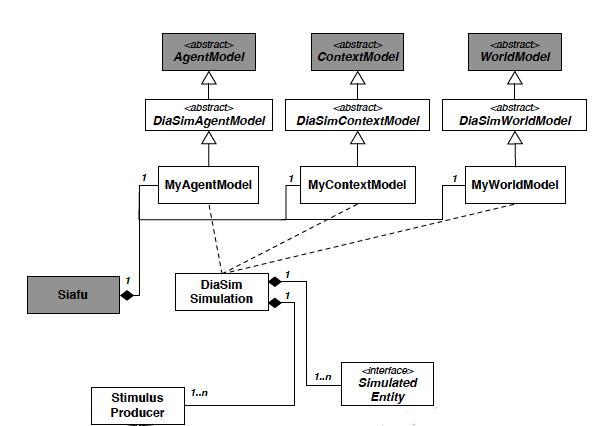
\includegraphics[width=\linewidth]{gfx/Chapter2/diasim_and_siafu}
	\caption{DiaSim and Siafu}
	\label{fig:diasim_and_siafu}
\end{figure}

The simulated data is available in 2D graphical representation and through a web service interface. Using the current 2D interface, the agent can be moved around the environment and can be facing four directions. The simulated sensors and actuators trigger actions based on the agent's proximity and the current context of other monitored entities in the system. At the moment of writing this thesis, no other interactions are available within DiaSim; the agent cannot interact with devices by explicitly triggering actions, nor can it interact with physical objects.\\

Although limited at the moment, the researchers of DiaSim are planing, as future work, to enhance the interaction capabilities by visualizing the simulation in a 3D engine.
%END: DiaSim 

%BEGIN: UbiWise 
\section{UbiWise}\label{sec:ubiwise}
\emph{UbiWise, A Simulator for Ubiquitous Computing Systems Design.}\\

UbiWise \cite{barton2003ubiwise} is a device-centric simulator. The target of this work was to allow researchers to simulate ubiquitous computing devices\footnote{networked, context-aware devices} before physical prototypes are available. The purpose of this is to empower the researcher to write software for the device and test it from a user interaction's point of view, in the actual physical environment the device was envisioned to be used in. This project emerged from two independent simulators: UbiSim and WISE.\\

To give an example of devices simulated with UbiWise, in the evaluation they have presented a wireless digital camera and wireless picture frames. The camera could easily connect to one of the frames and transfer a digital picture to be displayed.\\

UbiSim is a 3D environment simulator, aimed at producing context information in real-time, in a close to realistic environment. To simulate the environment, they have used the Quake III Arena (Q3A)\footnote{\url{http://www.idsoftware.com/gate.php}} first person shooter gaming engine, written in the C programming language. On top of the raw simulated data outputted by Q3A, they have built a \emph{context server} which processes the simulated data and delivers meaningful context data to external applications and services. The simulator is also able to process data from sensors in the real-world, generating mixed reality together with the simulated data.\\

WISE is a 2D device interaction simulator written in Java. This allows the user to interact with the software running on the device, interacting with real-world web services and other simulated devices.\\

In the 3D physical environment, the set of simulated devices are used in a context-aware manner, reacting to physical events and contextual changes. The devices might be portable, hand-held by a virtual agent the user controls (e.g. a digital camera enhanced with Internet connectivity) or they might be static devices, attached to a physical entity (e.g. a wireless enhanced picture frame on a wall). The simulation monitors the proximity between the devices, triggering events and allowing the software running on the devices to take specific actions.

In the 2D environment, the set of devices are presented in desktop-alike windows and they react to mouse clicks and network events. This allows to user to directly interact with the device through the simulated interface. Figure \ref{fig:ubiwise_2d_view} depicts a screenshot of the 2D view.\\
\begin{figure}[H]
	\centering
	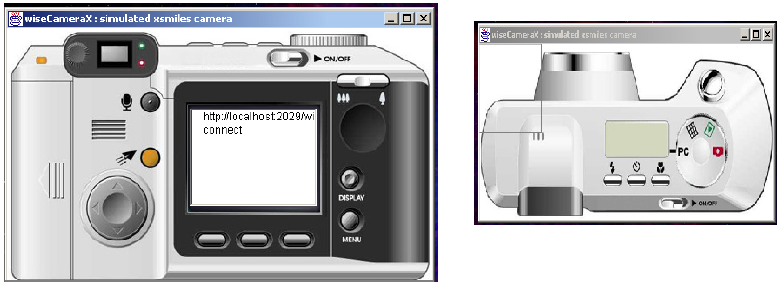
\includegraphics[width=\linewidth]{gfx/Chapter2/ubiwise_2d_view}
	\caption{UbiWise 2D view to interact with devices}
	\label{fig:ubiwise_2d_view}
\end{figure}

The simulator was developed on top of 3D game engine, empowering the agent to freely walk around the simulated environment. As the framework is device centric, the interaction between the agent and the environment is focused on interacting with the simulated devices: ''the simulator concentrates on computation and communications devices
situated within their physical environments.'' \cite{barton2003ubiwise}. One of the devices might be hand-held and carried around by the agent. There is no mention in the paper about the ability of the agent to put the hand held device down or to pick up another one. Physical objects are part of the environment, but they are not monitored and their state is not part of the system's context data. Figure \ref{fig:ubiwise_3d_view} presents a screenshot of the 3D view.\\
\begin{figure}[H]
	\centering
	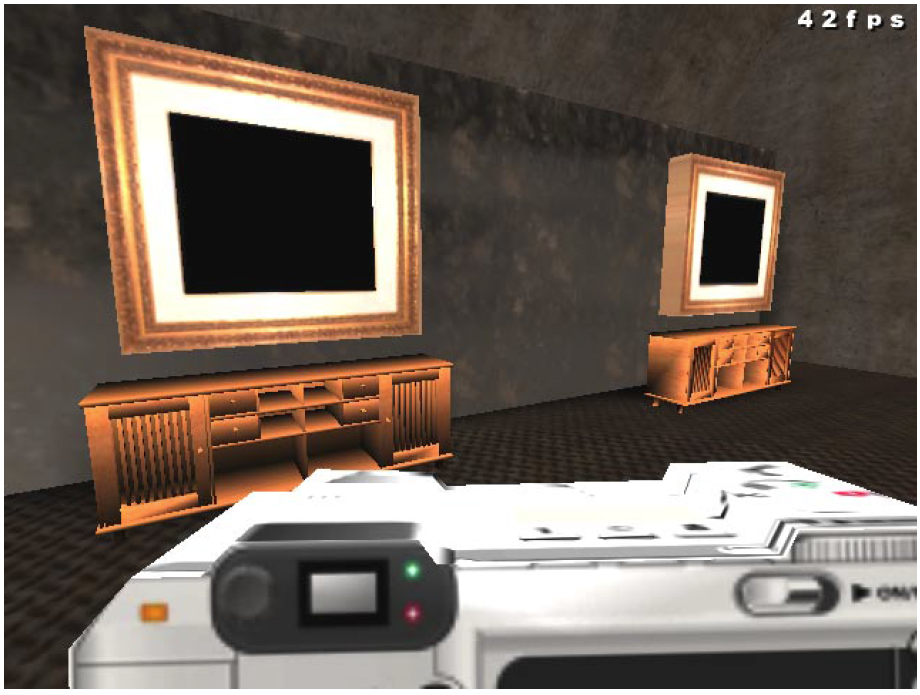
\includegraphics[width=\linewidth]{gfx/Chapter2/ubiwise_3d_view}
	\caption{UbiWise: 3D view of the physical environment}
	\label{fig:ubiwise_3d_view}
\end{figure}

UbiWise empowers the researcher to write actual software that runs on the simulated devices. The framework monitors proximity of the agent towards devices and proximity of the devices to each other, making this information available, together with other contextual data, to the software running on the devices.\\

The framework's source code is publicly available.
%END: UbiWise

%BEGIN: Tatus
\section{TATUS}\label{sec:tatus}
\emph{A Testbed for Evaluating Human Interaction with Ubiquitous Computing Environments}\\

Tatus \cite{o2005testbed} is as a ubiquitous computing simulator aimed at overcoming the challenges of effectively evaluating human interaction with adaptive ubiquitous technologies. These challenges are mainly imposed by the cost and logistics of building and controlling the context in such real-life environments. In other words, TATUS is a simulator supporting research and development of adaptive software controlling ubiquitous computing environments.\\

Figure \ref{fig:tatus_overview} depicts the high-level overview of the simulator. We can identify two main components: the 3D Simulated Ubiquitous Computing Environment and the System Under Test (SUT).\\

\begin{figure}[H]
	\centering
	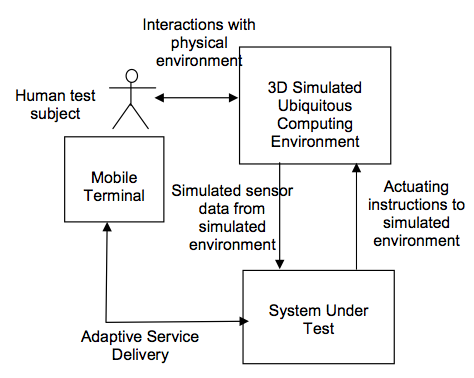
\includegraphics[width=\linewidth]{gfx/Chapter2/tatus_system_overview}
	\caption{TATUS: High-level simulator overview}
	\label{fig:tatus_overview}
\end{figure}

The 3D simulator was implemented on top of the Half-Life\footnote{\url{http://www.valvesoftware.com}} Game Engine's software development kit (SDK), written in C/C++. Half-Life is a 3D first-person-shooter network game. It is implemented based on client-server architecture with multi-player capabilities (up to 32 players simultaneously). Choosing this game engine was meant to provide a realistic user experience. Figure \ref{fig:tatus_simulated_meeting_room} presents a screenshot of a running simulation.\\

\begin{figure}[H]
	\centering
	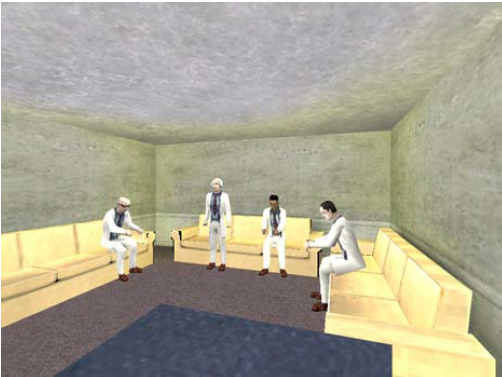
\includegraphics[width=\linewidth]{gfx/Chapter2/tatus_simulated_meeting_room}
	\caption{TATUS: Simulated meeting room with multiple characters}
	\label{fig:tatus_simulated_meeting_room}
\end{figure}

The actual simulated environment is created using a map editor from Valve called Hammer (a drawing tool for building maps). This can be used to generate complex and realistic environments as the tool offers a wide range of graphical editing possibilities. The SDK is then able to load a simulated environment's physical settings from the files generated by the map editor.\\

To simulated sensors and actuators they have exploited a concept called \emph{Triggers} from the SDK. They are used to generate associated events based on a player's movements and location. The state of these triggers together with the agents location at a certain point in time represent the state of the simulated environment. To allow easy access to the data, the simulator exposes an API which offers both querying and modifying capabilities. Queries allow to select certain aspects of the current state based on various parameters, whereas through modifications the SUT can impose changes on the simulated environment.\\

A SUT is written as independent pieces of software. It can even run on a separate machines, while multiple SUTs can connect simultaneously to the same simulator. To allow SUTs to run on separate machines the simulator has embedded networking capabilities and communicates through messages. Outgoing messages carry state information, while incoming messages carry instructions to modify the simulated environment. Moreover, to abstract out the network interaction from the SUTs, the simulator provides a Proxy making the communication from the test software's side easier.\\

As the simulator was developed on top of 3D game engine, it empowers the agent to freely walk around the simulated environment, while the interaction is based on proximity only. This means that entities will take a specific action when the agent is detected nearby; ''when a player enters a region of a map occupied by a trigger
the associated event is activated e.g. a door is opened'' \cite{o2005testbed}. These triggers can be attached to both physical objects and devices, enabling both categories of objects to be interacted with, as such.\\

The framework exposes an API so that third party software can easily access and modify the context data within the ongoing simulation.
%END: Tatus

%BEGIN: DISCUSSION
\section{Discussions}\label{sec:discussions}

%Service in Smart Homes
% The framework presented in Section \ref{sec:services_in_smart_homes} is solely oriented towards emulating sensors withing a smart home. The system supports in the simulated environment both emulated sensors and representation of real-life sensory data. For the implementation of virtual stubs they have employed the service-oriented computing paradigm, which is widely used to implement systems requiring high interoperability, scalability, security and reliability. One of the main advantages is that such software can seamlessly integrate other systems written in other programming languages and even deployed under different operating systems.\\

% Although they have created a highly decoupled architecture, the framework is able to represent a very limited types of entities. The characteristics monitored by the framework for the entities and the simulated agent are limited to proximity only.\\

%Simulation of Smart Environments
In the simulation of smart environments \ref{sec:sim_of_smart_envs}, the eHomeSimulator design promotes loose coupling between components. The underlying framework's architecture offers good support for reusability of smart home services and integration with real-life devices. Sensor and devices are operated on a per room basis, not on actual proximity to each individual entity. Devices in the current room can be operated through the \emph{Control Panel} (e.g. turn lamp on/off). The simulated entities are static (the agent can't move them). Actually, all the agent can do is move from room to room, this will trigger sensors to be activated/deactivated, which in turn might might change the state of other entities. There is no support for mobility of devices, nor is it in plan for future work. Moreover, the user can manipulate the agent (the virtual avatar), to walk around in the 2D environment. Given the nature of the visualization, the agent can be facing four directions: forward, backward, left or right.\\

The project is close sourced, making it impossible to extend, to reuse or to contribute to it. In conclusion, the simulator is target solely on simulating sensors in a smart home and how the presence of the human agent influences the environment. The framework was not designed to simulate the environment from the human agent's point of view, it was rather designed to simulated the evolution of sensors based on the human agent's presence. From this project's perspective, eHomeSimulator is outdated, imposing a limited number of interaction possibilities. That is why I am not be including it in further discussions.\\

% \begin{table}[H]
% 	\begin{center}
% 		\small \begin{tabular*}{1.1\columnwidth}{lllll}
% 			\\ \hline \hline
% 			Characteristics & Simact & DiaSim & Tatus & Ubiwise \\ \hline \hline

% 			Support for physical objects? & yes & yes & yes & yes \\ \hline
% 			Support for devices? & yes & yes & yes & yes \\ \hline
% 			Simulate software running on devices? & no & no & no & yes \\ \hline
% 			Support of object composition? & yes & yes & yes & yes \\ \hline
% 			Wearable devices? & no & no & no & no \\ \hline
% 			Receive data from real-life sensors? & yes & yes & no & yes \\ \hline

% 			Monitors agent location? & yes & yes & yes & yes \\ \hline
% 			Visual spectrum of the agent? & yes & no & yes & yes \\ \hline
% 			Audio spectrum of the agent? & yes & no & yes & yes \\ \hline
% 			Body position (crouching/standing)? & yes & no & yes & yes \\ \hline
% 			Pick up object & no & no & no & no \\ \hline
% 			Carry object around & no & no & yes & yes \\ \hline
% 			Put object down & no & no & no & no \\ \hline
% 			Object in agent's hand & no & no & yes & yes \\ \hline
% 			Object in agent's pocket/backpack & no & no & no & no \\ \hline

% 			Agent interaction with devices & no & no & no & yes \\ \hline

% 			Is open sources?             & yes & no & no & yes \\ \hline
% 		\end{tabular*}
		
% 		\caption{Features comparison}
% 		\label{table:comparison}
% 	\end{center}
% \end{table}

Table \ref{table:comparison} depicts the characteristics of interest for the current work, highlighting whether or not they are implemented within the system from the related work.

\begin{table}[H]
	\begin{center}
		\small \begin{tabular*}{1.1\columnwidth}{p{6.5cm}llll}
			\\ \hline \hline
			Characteristics & Simact & DiaSim & Tatus & Ubiwise \\ \hline \hline

			Visual representation of the simulated environment & yes & yes & yes & yes \\ \hline
			Interact with the environment through a virtual avatar & no & yes & yes & yes \\ \hline
			360\textdegree control of the avatar & no & no & yes & yes \\ \hline
			Simulate sensors & yes & yes & yes & yes \\ \hline
			Directly interact with physical objects & yes & no & no & no \\ \hline
			Interact with physical objects using attached sensors & yes & yes & yes & yes \\ \hline
			Interact with devices (mediators) & yes & yes & yes & yes \\ \hline
			Interact with software (virtual objects) & no & no & no & yes \\ \hline
			Pick objects up & no & no & no & no \\ \hline
			Put objects down & no & no & no & no \\ \hline
			Carry objects around & no & no & no & yes \\ \hline
			Monitors the agent's location & no & yes & yes & yes \\ \hline
			Visual spectrum of the agent \footnote{Objects within to the agents sight} & no & no & yes & yes \\ \hline
			Classify objects based on agent proximity & no & no & no & no \\ \hline
		 	Provides API for third party services to access context data & yes & no & yes & no \\ \hline
		 	Is open source? & yes & no & no & yes \\ \hline
		\end{tabular*}
		
		\caption{Features comparison}
		\label{table:comparison}
	\end{center}
\end{table}

%Diasim
After thorough analysis, I found DiaSim's \ref{sec:diasim} simulation model as being generic enough to possibly host our needs. The simulation model seems to be flexible and open for further modifications. But, the system is not open source and the research team is not yet open for external collaboration.\\

Even if building on top of DiaSim would have been possible, some outstanding issues should be tackled. The simulated environment does not monitor the agent's visual spectrum (objects within to the agents sight). To accommodate this need, the renderer module should be entirely replaced. Besides, there is no support for direct interaction with physical and virtual objects. The only type of interaction is proximity based: i.e. a sensor attached to a door would command the door to open if the agent is within range. Moreover, DiaSim is also lacking an open API to enable third party service to make use of the simulated system's context data.\\

In conclusion, DiaSim offers great support for setting up a new simulation of a sensor-enhanced environment, from scratch. It simulates the evolution of the environment over time, influenced by the presence of one or many agents. But, it lacks support for the body-centric approach of the current work.\\

%Simact
SIMACT came up with a slightly different approach. The entire simulation is controlled by the framework as it interprets the simulation scenario, described in an XML file. This is a step-by-step description of how various parameters of the system (e.g. the temperature in a room) and of objects (e.g. door opened/closed, lamp on/off) evolve. SIMACT is oriented towards observing the systems evolution over time with the ability to control the execution of the steps in a fine grained manner: pause, resume, go back, etc. As the simulation is running, it is animated in 3D view.\\

This approach comes with a drawback: SIMACT does not implement the concept of an avatar. The researcher is enabled to move a camera around, zoom in and zoom out in order to find the best spot to observe the animation of the ongoing simulation. The animation was implemented using the JMonkey game engine. This game engine has to offer more than just rendering capabilities, it allows to implement the concept of an agent offering components to implement movement and interaction with the environment. In Chapter \ref{ch:design} I will argue for JMonkey as a possible candidate to be used in my work.\\

Although the framework is released as open-source \cite{bouchard:simact:Online} under GPLv3 \cite{gpl:v3}, it was written in french! (continue!)

%Tatus
In Tatus \ref{sec:tatus}, the context-awareness is limited to sensors and actuators reacting to the user's position. This is actually not that bad because in the game engine SDK the developer can extract the position of entities, determine proximity of other entities within a given radius and determine the presence of other entities within a field of view. All these data helps to implement simulations for a wide range of sensors.\\

The user control provided by the game engine is pretty advanced allowing the agent to move in any direction, crouch, jump, sit etc. This is a big plus as it adds a good sense of reality to the game.\\

Multiple users can join and experience the same simulated environment at the same time. Not all players have to be human, non-player-characters (controlled by the AI of the engine) can be present as well.\\

One of the main challenges in developing the simulator was that the learning curve of the SDK, in order to extend it, was difficult and time-consuming. But, as a result, they have tried to provide a flexible simulation environment where researchers can easily simulate other environments without the need to modify any SDK level code.\\

Unfortunately the simulator is not open-source so making it unusable for research outside the institution it was developed in.\\

%Ubiwise
Although UbiWise \ref{sec:ubiwise} was released under LGPL\cite{lgpl}, offering the software to the open-source community, it presents two main issues from the perspective of my work. The first aspect is that it is oriented towards emulating device protoypes making it hard to emulate custom sensors. The second challenge is the learning curve it takes to get started with it. In order to customize it to a certain area, one would need to dive deep into the Q3A engine code, which is hard, tedious and time consuming task.\\
%END: DISCUSSION